\section{Evaluation of Existing Methods}
\subsection{Baseline Considerations}
We recall that the work of CodeMirage\cite{guo2025codemirage} was 
not only to provide a dataset, but also to perform 
tests on some of the methods present in the literature.

The methods tested by CodeMirage can be divided into 4 categories:
\begin{enumerate}
    \item \textbf{Zero-shot detectors}: 
    These are methods based on the computation of code-related metrics and do not require any training.
    \newline The advantage of these methods is that they are totally independent of any dataset 
    and therefore “immune” to the \textit{out-of-domain effect}. This characteristic is very useful 
    if the detection method must be per-formant in different domains. 
    \newline Unfortunately, these methods also turn out to be complicated to develop 
    because they require a deep analysis of every type of code generated by an LLM, 
    unless such characteristics exist and are detectable by a non-AI-based method. 
    \newline Moreover, it is essential to identify characteristics that depend intrinsically on the 
    architecture of LLMs and not on their training, otherwise these methods would 
    become even less reliable over time than machine-learning-based methods.

    
    \item \textbf{Embedding-based detectors}: 
    These methods consist of using an encoder-only transformer 
    (or one that can be used as such), trained on code and not 
    fine-tuned for the classification task, paired with a classifier 
    trained on a dataset of LLM and human code.
    \newline These methods always remain inferior to the performance achieved by the next category.
    
    \item \textbf{Fine-tuned detectors}: 
    Fine-tuned methods are like embedding methods, but during training they 
    also train the encoder-only. The difference between the various methods 
    lies only in the choice of the encoder-only model. They seem to be the 
    models that in general achieve the best performance but are also the most 
    affected overall by the out-of-domain effect.
    
    \item \textbf{Pretrained LLM with downstream detector}:
    The last category is a middle ground between the previous ones and seems to 
    suffer overall less from out-of-domain problems. This category statistically 
    analyses the output of an LLM to which the code has been provided via a prompt, 
    such as \texttt{“explain this code:\{code\}”}. Such statistical 
    features are used by a classifier to learn which ones identify 
    human code more and which ones identify 
    LLM code.
\end{enumerate}

\subsubsection{First results}

\begin{figure}[H]
    \centering
    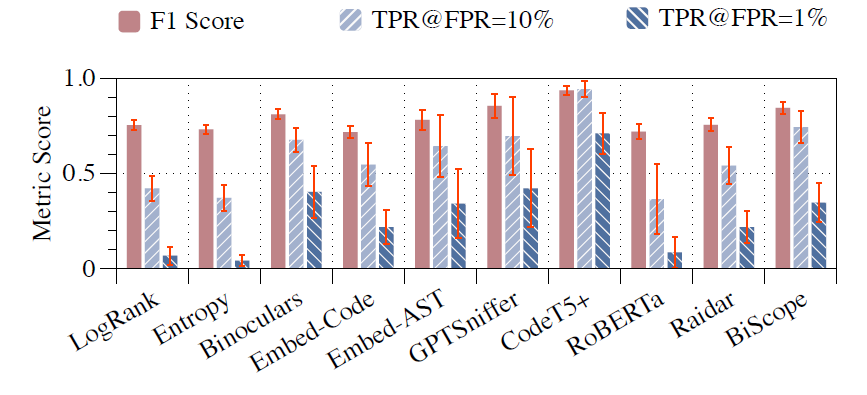
\includegraphics[width=1\textwidth]{img/CodeMirage/tests.png}
    \caption{CodeMirage's tests}
    \label{fig:CodeMirage-tests}
\end{figure}

The presented methods therefore fall into the previously described categories:
Zero-shot detectors: logRank\cite{gehrmann2019gltr}, entropy\cite{lavergne2008detecting}, 
binoculars\cite{hans2024spotting}.
Embedding-based detectors: Embed-Code, Embed-AST.
Fine-tuned detectors: GPTSniffer\cite{nguyen2024gptsniffer}, CodeT5+\cite{wang2023codet5+}, RoBERTa\cite{liu2019roberta}.
Pretrained LLM with downstream detector: Raidar\cite{mao2024raidar}, Bioscope \cite{guo2024biscope}.


Furthermore, these tests are not complete: 
recall that the CodeMirage dataset includes 
only code coming from GitHub and tends to be 
large. In addition, (more importantly), 
they never mention having removed comments in the code, 
which not infrequently (by analysing the dataset) appear 
to be extremely long and verbose. For this reason it is 
plausible that zero-shot methods designed for natural text 
apparently achieve good results on code as well 
(contrary to what many other works state: 
\textit{ zero-shot text detectors are ineffective in detecting code, 
likely due to the unique statistical properties found in code structures.}
\cite{yang2023zero}
).

It is important to make some clarifications: all the zero-shot 
methods presented were designed to analyze natural text which, 
as previously stated, is a process extremely different from 
analyzing code due to the naturally low next-token perplexity 
(a feature on which almost all zero-shot methods are based). 
The Embed-Code and Embed-AST methods are both based on 
CodeXEmbed-2B\cite{liu2024codexembed}, where in the first case code is provided and 
in the second case the AST obtained from code. GPTSniffer, 
CodeT5+, and RoBERTa are three methods that rely entirely on 
the GPTSniffer\cite{nguyen2024gptsniffer} technique and differ only by the encoder used. 
Finally, both Raidar and Bioscope are methods designed especially 
for natural text, but they seem to achieve good results on code as well.

For all the above reasons, it is justified not to stop at these tests but to pursue more in-depth analyses. In particular, additional methods not considered by CodeMirage and specifically designed for LLM code classification will be examined. Nevertheless, the CodeMirage results should not be ignored.

Key points: the method that appears to deliver the best performance 
is GPTSniffer with CodeT5+. BiScope also merits consideration. 
Rationale: CodeT5+ attains very high TPR at a 10\% 
FPR. However, these tests were run on a split of the 
CodeMirage dataset. Therefore, GPTSniffer with CodeT5+ 
was not evaluated out of domain, which is the main weakness 
of fine-tuned detectors, the category to which GPTSniffer with 
CodeT5+ belongs.

Similarly, BiScope belongs to the pretrained LLM with 
downstream detector category, which has fewer difficulties 
adapting to out-of-domain tests. It also achieves positive 
TPR at an FPR of 10\%. Therefore, GPTSniffer with 
CodeT5+ and BiScope will be considered the baselines 
for subsequent models.
\subsection{Test framework}
